\section{Evaluation}
\label{sec:eval}

\lstMakeShortInline[mathescape=true]{|}


We have implemented our technique for repairing type errors for a purely
functional subset of \ocaml with polymorphic types and functions. We seek to
answer the following Research Questions:

\begin{itemize}
    \item \textbf{RQ1}: What is the \emph{quality} of \toolname's repairs?
    \item \textbf{RQ2}: Do our ML models \emph{generalize} well for error
    localization and template prediction?
    \item \textbf{RQ3}: How do fix templates affect program repair?
    \item \textbf{RQ4}: Are \toolname's repairs actually useful to novice programmers
    for feedback generation?
\end{itemize}
\GS{associate them with subsections}

We first present our experimental methodology and then we will try to answer
each of the above questions, drawing from our results from a human study and our
manual evaluation.


\subsection{General Methodology}
\label{sec:eval:gen_method}
For our evaluation, we use an \ocaml dataset gathered from an undergraduate
Programming Languages university course, previously used in related work
\citep{yunounderstand,Seidel:2017}. It consists of erroneous programs and their
subsequent fixes and is divided in two parts; the Spring 2014 class (\SPRING)
and the Fall 2015 class (\FALL). The homework required students to write 23
distinct programs that demonstrate a range of functional programming idioms, \eg
higher-order functions and (polymorphic) algebraic data types.

\paragraph{Feature Extraction}
We extract 416 features from each sub-expression in a program, including:
%
\begin{enumerate}
  \item 45 local syntactic features.
  \item 315 contextual syntactic features. For each subexpression we
    additionally extract the local syntactic features of its first 4
    (left-to-right) children. In addition, we extract those features for its
    ancestors, starting from its parent and going up to two more parent nodes.
    % If an expression does not have a ancestor or children, these features will
    % simply be disabled. If an expression has more than four children, the
    % classifiers will receive no information about the additional children.
  \item 88 typing features. We support |int|s, |float|s, |char|s, |string|s, and
    the user-defined |expr|. These features are extracted for each
    sub-expression and its context.
  \item 1 feature denoting the size of each subexpression.
\end{enumerate}

\paragraph{Dataset cleaning}
We extract fixes as expressions replacements over a program pair using \diffsym.
A disadvantage of using \diffsym s with this dataset is that students may have
made many, potentially unrelated, changes between compilations; at some point
the ``fix'' becomes a ``rewrite''. These ``rewrites'' can potentially lead to
meaningless fix templates and error locations. We discard such outliers when the
fraction of subexpressions that have changed in a program is more than one
standard deviation above the mean, establishing a diff threshold of 40\%. We
also discard programs that have changes in 5 or more locations. Even
state-of-the-art multi-location repair techniques can't reproduce such ``fixes''
\citep{Saha_2019}. The discarded changes account for roughly 32\% of each
dataset, leaving 2,475 program pairs for \SPRING and 2,177 pairs for \FALL. In
all our evaluation, we use \SPRING as a training set and \FALL as a test set.

\paragraph{Accuracy Metrics}
Most developers will consider around five (or slightly more) suggestions before
falling back to manual debugging \citep{Kochhar2016-oc}. Therefore, we consider
\toolname's accuracy up to the \emph{top six} fix template prediction, \ie
predicted fix templates that represent the user's actual fix. We also include
the \emph{confusion matrix} of the each location's first prediction, to present
what templates our models usually mix together and see if they generalize well
between different groups of solutions.

\paragraph{Repair Quality}
Finally, for a more qualitative evaluation of \toolname's synthesized solutions
based on the above results, we carried out a human study at \emph{university
elided for blind review}. Each participant was asked to evaluate the quality of
the program fixes and their locations against a state-of-the-art baseline (the
\seminal's repair algorithm \citep{Lerner2007-dt}). For each program, beyond the
two repairs, participants were presented with the original ill-typed program,
along with the standard \ocaml compiler's error message and a short description
of what the original author of the program intended it to do. For a more
detailed description of the user study setup and evaluation, see
\autoref{sec:eval:qual_eval}.

\subsection{Quantitative Evaluation}
\label{sec:eval:quan_eval}

First, we evaluate the accuracy of our template predictions.


\subsubsection{Template Prediction Accuracy}
\label{subsec:eval:templ_acc}

\paragraph{Baselines}
We provide two simple baseline classifiers for the comparison: a random choice
of fix templates and predictions based on the templates' training set
popularity. Specifically:
\begin{description}
  \item[\random] A baseline classifier that \emph{uniformly} selects a fix
    template to return. There is no training necessary with this classifier.
  \item[\popular] This classifier returns always the most popular templates in
    the training set in decreasing order. The training phase of this classifier
    just includes learning the popularity of each template partition on the
    training set.
  \item[\textsc{Deep Neural Network} (\dnn)] A multi-layer neural network, that
    utilizes three fully-connected hidden layers of 512 neurons. The neurons use
    rectified linear units (ReLU) as their activation function.
\end{description}

A \dnn was trained using \emph{early stopping} \cite{Hastie2009-bn}, where the
training of a neural network is stopped when the accuracy on a distinct small
part of the training set is not improved after a certain amount of epochs. We
set that amount to 5 and the maximum number of epochs to 200. The \textsc{Adam}
optimizer \citep{Kingma2014-ng}, a variant of stochastic gradient descent that
has been found to converge faster, was used to train our \dnn.

% colors from http://colorbrewer2.org/?type=sequential&scheme=Blues&n=3
\definecolor{blue1}{HTML}{DEEBF7}
\definecolor{blue2}{HTML}{9ECAE1}
\definecolor{blue3}{HTML}{3182BD}
\definecolor{green1}{HTML}{E5F5E0}
\definecolor{green2}{HTML}{A1D99B}
\definecolor{green3}{HTML}{31A354}

\begin{figure}[t]
\centering
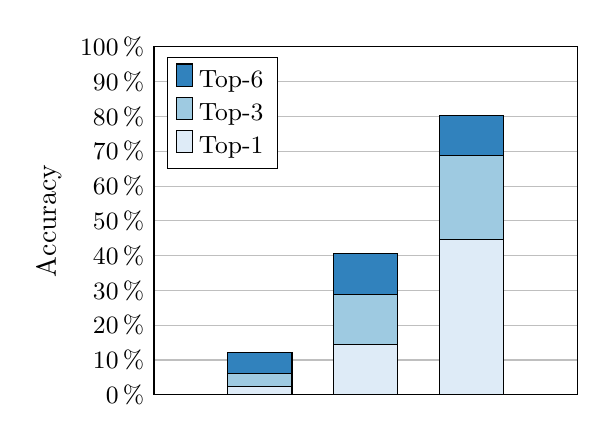
\begin{tikzpicture}
\begin{axis}[
  ybar stacked,
  % width=\linewidth,
  height=6cm,
  % title={Accuracy of Repair Template Prediction},
  ylabel={Accuracy},
  bar width=0.82cm,
  ymin=0.0,
  ymax=100.0,
  ytick={0.0, 10.0, 20.0, 30.0, 40.0, 50.0, 60.0, 70.0, 80.0, 90.0, 100.0},
  yticklabel={\pgfmathparse{\tick}\pgfmathprintnumber{\pgfmathresult}\,\%},
  ytick style={draw=none},
  ymajorgrids = true,
  symbolic x coords={random, popular, dnn},
  enlarge x limits=0.5,
  xtick=data,
  xtick style={draw=none},
  xticklabels={\random, \popular, \dnn},
  %x tick label style={rotate=45, anchor=north east},
  x tick label style={font=\small},
  y tick label style={font=\small},
  reverse legend,
  transpose legend,
  legend style={legend pos = north west, legend columns=4, font=\small},
]

\addplot[draw=black, fill=blue1] coordinates {(random, 2.35646958011996552) (popular, 14.438731790916881) (dnn, 44.64438731790917)};
\addlegendentry{Top-1}
\addplot[draw=black, fill=blue2] coordinates {(random, 3.6846615252784924) (popular, 14.395886889460153) (dnn, 24.250214224507282)};
\addlegendentry{Top-3}
\addplot[draw=black, fill=blue3] coordinates {(random, 6.212510711225363) (popular, 11.825192802056556) (dnn, 11.482433590402735)};
\addlegendentry{Top-6}

\end{axis}
\end{tikzpicture}
\caption{
  Results of our template prediction classifiers using the \emph{50 most
  popular} templates. We present the results up to the top 6 predictions, since
  our synthesis algorithm considers that many templates before falling to a
  different location.
}
\label{fig:accuracy-results}
\end{figure}


\begin{figure}[t]
  \centering
  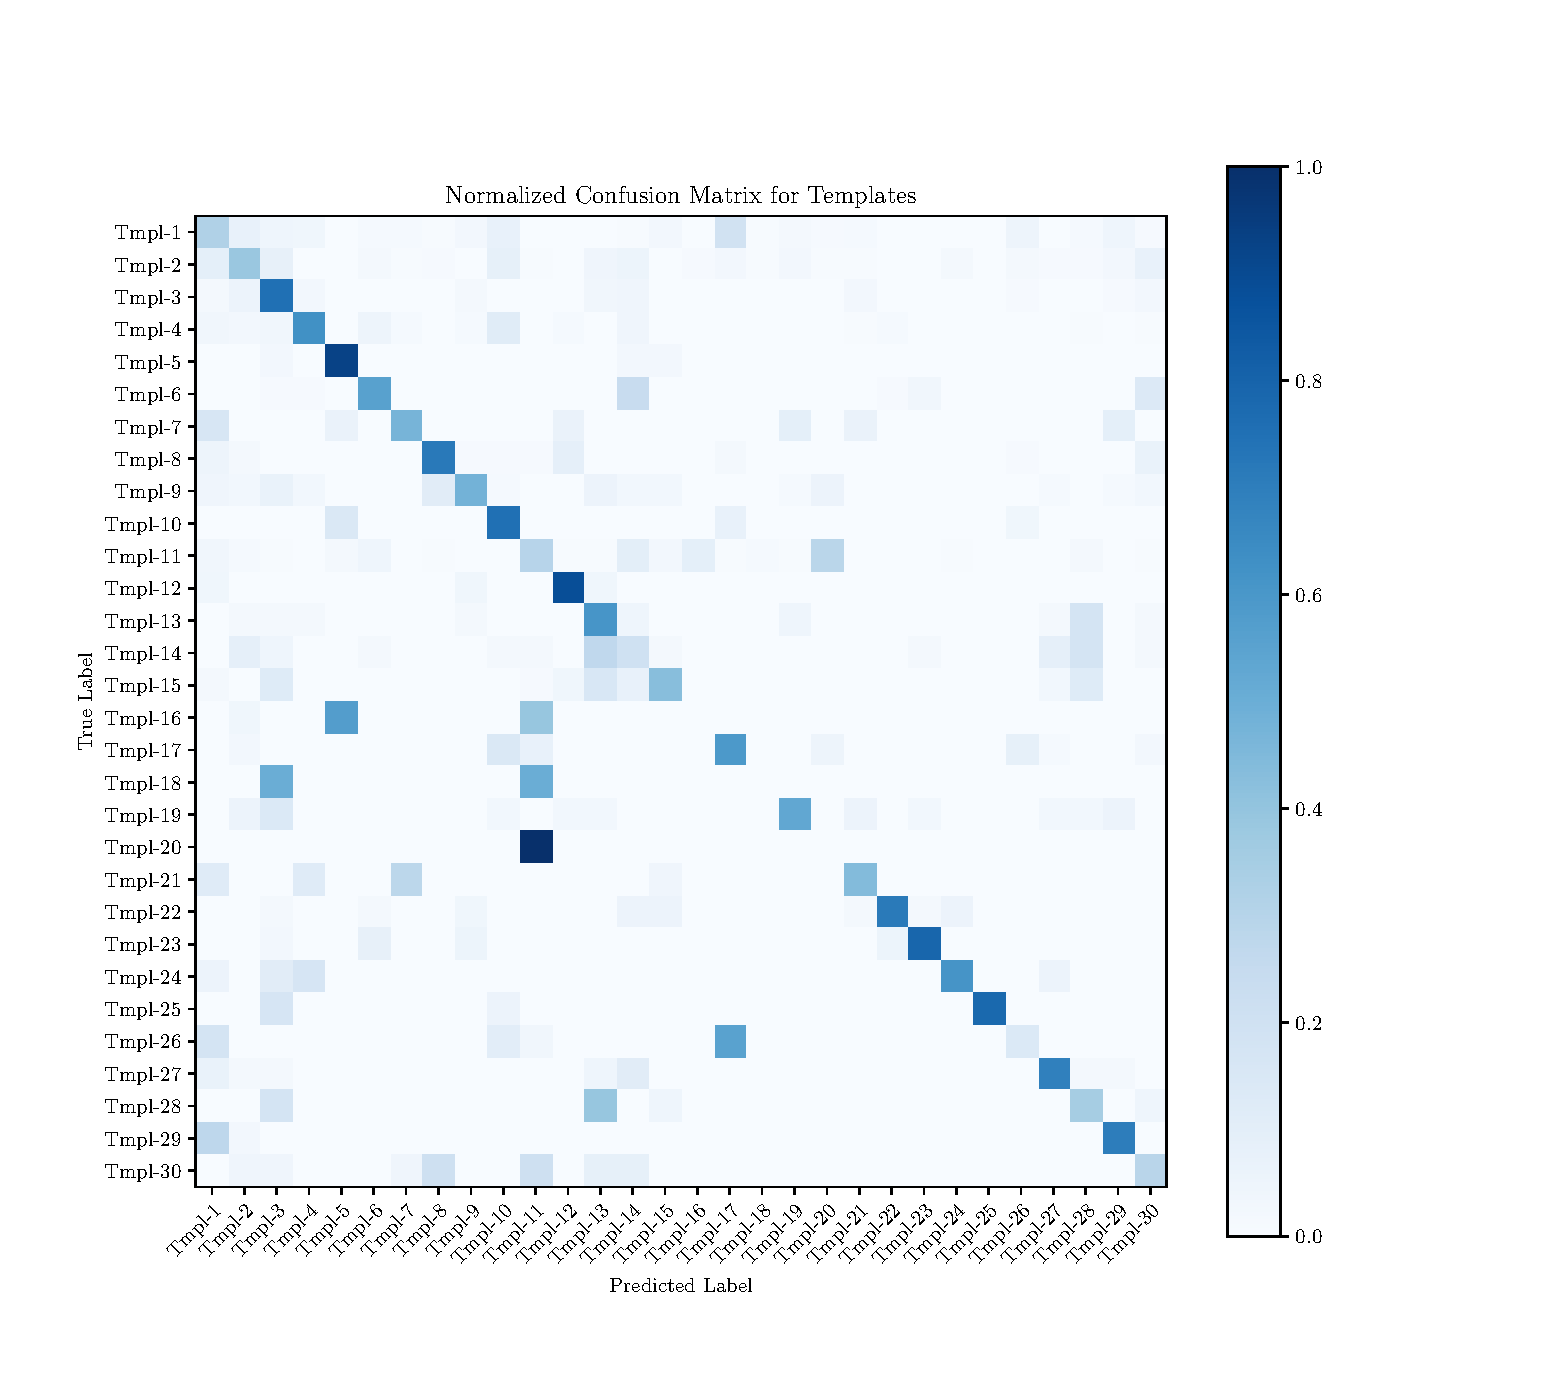
\includegraphics[trim={30 40 100 70},clip,width=\linewidth]{evaluation-conf-matrix.pdf}
  \caption{The confusion matrix of the \emph{top 30} templates. Bolder parts of
  the heatmap show templates that are often mis-predicted with another template.
  The bolder the diagonal is, the more accurate predictions we make.}
  \label{fig:conf-matrix}
\end{figure}

\paragraph{Results}
\autoref{fig:accuracy-results} shows the accuracy results of our template
prediction experiments. The naive baseline of selecting templates at random
achieves \RandomTopOne\% Top-1 accuracy (\RandomTopSix\% Top-6), while the
\popular classifier achieves a Top-1 accuracy of \PopularTopOne\%
(\PopularTopSix\% Top-6). Our \dnn classifier significantly outperforms those
naive classifiers, ranging from \DnnTopOne\% Top-1 accuracy to \DnnTopSix\%
Top-6 accuracy. Interestingly, with only \dnn's first prediction, one
outperforms top 6 predictions of both \random and \popular.

The \random classifier selects \emph{randomly} a template, out of the 50 learned
ones from the \SPRING training dataset, for each location it is presented. Its
low performance is expected. \popular performs better on our dataset: some
homework assignments were shared between \SPRING and \FALL quarters and, while
different groups of students solved these problems for each quarter, the novice
mistakes that they made seem to have a \emph{pattern}. Thus, the most
\emph{popular ``fixes''} (and therefore the relevant templates) that were
applied to \SPRING, are also popular in \FALL. However, the almost \emph{2x
higher} accuracy of our \dnn classifier shows that we can learn \emph{better
patterns} from these datasets and that our \dnn model is able to
\emph{generalize} between different solutions of the problems.

\autoref{fig:conf-matrix} further demonstrates that our \dnn generalizes well.
This Figure includes the confusion matrix of the top 30 templates that were
acquired from the training set and were tested on the same \FALL dataset as
before. We observe that most of the templates are predicted correctly and only a
few of them are often mis-predicted for another template. For example, we see
that programs that would require template 20 to be fixed almost always are
mis-predicted with template 11.

\GS{show those two templates, both ``let''s with some ``tuple'' in their ASTs}

% \subsubsection{Error Localization Accuracy}
% \label{subsec:eval:error_loc_acc}

% \paragraph{Method}
% For our error localization task, we again train a multi-layer neural
% network, with the same hyper-parameters as in \ref{subsec:eval:error_loc_acc}. Our
% network firstly uses two fully-connected hidden layers of 1024 neurons and one
% of 512 neurons before the output layer. The neurons again use rectified linear
% units (ReLU) as their activation function and are trained using the \emph{early
% stopping} approach and the \textsc{Adam} optimizer.
% \WRW{notes: this paragraph feels repetitive: didn't we just say this a few
% paragaphs ago? Search for Adam.}

% Previous work \citep[][]{Seidel:2017} has used more shallow neural networks, but
% also fewer features per node. In our implementation, we added more contextual
% features following recent research direction, which has shown them to be the
% most important \citep[TODO: add the lstm paper][]{Seidel:2017}. Thus, we
% chose deeper neural network architectures for our error localization models as
% well.

% \begin{table}
%   \centering
%   \begin{tabular}{l|rr}
%     Classifier & Top-3  & Top-5 \\
%     \hline
%     \random   & 39.70\% & 58.73\% \\
%     \toolname & 79.71\% & 88.83\% \\
%   \end{tabular}
%   \caption{Experimental results of \toolname's error localization accuracy.
%   FIXME: We had Top-1, Top-3 and Top-6 in the last subsection. Why are we suddenly
%   Top-3 and Top-5 now? If we have the data available, can we be more
%   consistent?
%   }
%   \label{tab:err_loc_acc}
% \end{table}

% FIXME: It looks like we don't have any text yet that references
% tab:err\_loc\_acc. We need text that references the table: we cannot just
% have the table floating free. Walk the reader through the result.

\subsubsection{Empirical Repair Quality Evaluation}
\label{subsec:eval:man_rep_qual_eval}

\paragraph{Synthesis Algorithm}
We guide our synthesis algorithm, using fix template and location predictions.
Every program is given a timeout of \emph{60s} to be repaired by the synthesis
algorithm. Any program that takes more than that to synthesize can't have any
practical use for novices~\cite{FIXME}. In \autoref{tab:rite_naive}, we show two
instances of \toolname. \toolname refers to the implementation we have described
so far in this paper. The \naive implementation ignores the predicted fix
templates and only uses the predicted error locations to synthesize repairs.
This equivalent to \toolname where the fix templates are given just as program
holes $\_$.

The first column of \autoref{tab:rite_naive} shows how many programs were
completed on the time limit, while the second column how many returned a
type-correct solution. We observe that using fix templates for synthesis
actually allows more programs to return type-correct solutions. We also observe
that for the programs that are completed within the time limit, \toolname needs
an average of $8.81$ seconds to repair am erroneous program, while \naive takes
11.72seconds, a \textbf{33\%} increase.

The 11.85\% of the programs that fail to be repaired within that amount of time
fall in the case of the combined failure of our predictive models to give high
confidence scores to the correct locations and templates, thus making synthesis
very expensive.

% However, for the 87.46\% of the programs that finish
% synthesizing, around \textbf{96.32\%} return a solution that type-checks. The
% remaining 3.78\% for which no well-typed solution is produced usually required
% larger changes (\ie expressions whose ASTs were deeper than 4 levels).

% The average solution production time
% was \textbf{9.26s}. Of the well-typed solutions scenarios, almost
% \textbf{11\%} produced a repair identical to the historical human one
% within the top 3 repairs. This is considerable, because even non-identical
% repair suggestions can be quite helpful~\cite{FIXME}, and identical
% repair suggestions reduce novice effort~\cite{FIXME}.
% Our models can learn and capture novice intent in bug fixing.

% FIXME: \WRW{thinks this subsection is quite weak. We seem to be spending all
% of the time talking about what we fail or timeout at or giving excuses for
% why our numbers are small. We're burying the lead.}

\begin{table}
  \centering
  \begin{tabular}{l|ccc}
    Classifier & Completed & Repair Rate & Time (sec) \\
    \hline
    \naive   & 77.86\% & 74.78\% & 11.72 \\
    \toolname & 88.15\% & 84.80\% & 8.81 \\
  \end{tabular}
  \caption{Experimental results of \toolname's synthesis.}
  \label{tab:rite_naive}
\end{table}

\GS{here the \seminal - \toolname - \naive comparison}

\subsection{Qualitative Evaluation: User Study}
\label{sec:eval:qual_eval}

To assess the quality of \toolname's repairs, we conducted an online human
study with 29 participants. From this study, we found that both the edit
locations and final repairs produced by \toolname were better than those
produced by \seminal~\citep{Lerner2006-pj, Lerner2007-dt}, a state-of-the-art
Ocmal repair tool, in a statistically significant manner.
Subsection~\ref{subsec:eval:qual_study_setup} describes our experimental design,
and subsection~\ref{subsec:eval:study_res} presents our detailed findings.

\subsubsection{User Study Setup}
\label{subsec:eval:qual_study_setup}

Study participants were recruited from \emph{two public research
institutes removed for blind review}. The study was also advertised on Twitter.
To be included for analysis, participants had to assess the quality of, and give
comprehensible bug descriptions for, at least 5 / 10 stimuli. The study took around
25 minutes to complete. For compensation, participants had the option to enter a
drawing for an Amazon Echo voice assistant. In total, there were
29 valid participants.

To create the stimuli, a corpus of 21 buggy programs were randomly selected from
1834 type-correct synthesized programs in our dataset. From this corpus, each
participant was then shown 10 randomly-selected programs. Along with each buggy
program, participants were also shown two candidate repairs: one generated by
\toolname and one by \seminal. For both algorithms, we used the highest-ranked
solution returned. Participant were always unaware which tool generated which
candidate patch. Participants were then asked to assess the quality of each
candidate repair on a Likert scale of 1 to 5. They were further asked for a
binary assessment of the quality of each repair's edit location.
We also collected self-reported estimates of both programming and
\ocaml-specific experience as well as qualitative data assessing factors
influencing each participant's subjective judgment of repair quality.
From the 29 participants, we collected 554 patch quality assessments, 277 each
for \toolname and \seminal generated repairs.

%\begin{figure}
%  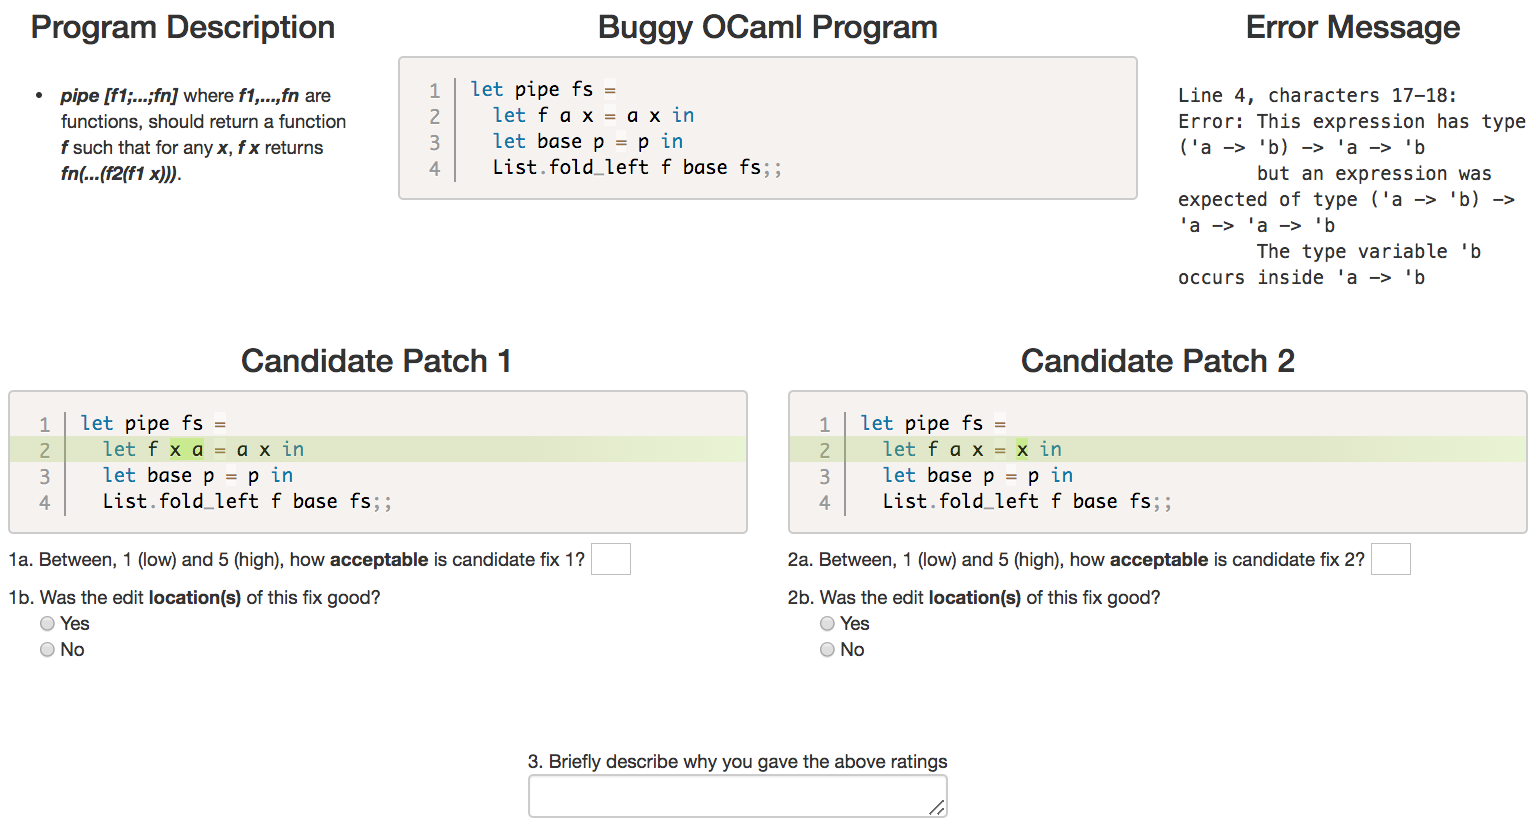
\includegraphics[width=8cm]{SampleStimuli.png}
%  \caption{A sample stimulus used for assessing repair quality.}
%  \label{fig:stimulus}
%\end{figure}

\subsubsection{Human Study Results}
\label{subsec:eval:study_res}

In a statistically significant manner, humans perceive that
\toolname's fault localization and final repairs are both of higher quality
than those produced by \seminal ($p=0.030$ and $p=0.024$
respectively)~\footnote{All tests for statistical significance used the
Wilcoxon signed-rank test.}.

Regarding fault localization, we find that humans agreed with \toolname-identified
edit locations 81.6\% of the time but only agreed with those of \seminal 74.0\%
of the time. This 10\% increase is important because
FIXME: You should explain why this matters.

As for the final repair, humans also prefer \toolname's patches
to those produced by \seminal. Specifically, \toolname's repairs achieved an
average quality rating of 2.41/5 while \seminal's repairs had an average rating
of only 2.11/5, 14\% increase ($p=0.030$).
FIXME: Spend more time talking about this success. Draw the conclusion
for the reader that you are doing better than previous work ina
statistically-significant manner. Indicate that 15\% better is still very
useful for students, perhaps by citing something.

\begin{figure*}
\begin{subfigure}[t]{.38\textwidth}
\begin{center}
\textbf{Programming Task:}
\end{center}
\texttt{wwhile(f, b)} should return $x$ where
there exist values $v_0,...,v_n$ such that:
$b = v_0$, $x = v_n$, and
for each $i$ between 0 and $n-2$, we have $f v_i = (v_i+1, true)$
and $f v_n-1 = (v_n, false)$.
\begin{center}
\textbf{Buggy Student Solution:}
\end{center}
\begin{compactcode}
let rec wwhile (f, b) =
let (b', c') = f b in if c' = true
then wwhile __(f b')__ else b';;
\end{compactcode}
\begin{center}
\textbf{\toolname Repair:}
\end{center}
\begin{compactcode}
           ...__(f, b')__...
\end{compactcode}
\begin{center}
\textbf{\seminal Repair:}
\end{center}
\begin{compactcode}
     ...__((f b'); [[...]]))__...
\end{compactcode}
\caption{Humans perceived \toolname's repair to be
better than \seminal ($p=0.002$): With 12 responses, \toolname's
repair had a mean score of 4.5/5 compared to \seminal's
score of 1.1/5.}
\label{subfig:good1}
\end{subfigure}\hfill
\begin{subfigure}[t]{.1\textwidth}
\end{subfigure}\hfill
\begin{subfigure}[t]{.28\textwidth}
\begin{center}
\textbf{Programming Task:}
\end{center}
\texttt{clone x n} should return a list of
\texttt{n} copies of the value \texttt{x}.
\begin{center}
\textbf{Buggy Student Solution:}
\end{center}
\begin{compactcode}
let rec clone x n =
if n <= 0 then []
else x :: __(clone (n - 1))__;;
\end{compactcode}
\begin{center}
\textbf{\toolname Repair:}
\end{center}
\begin{compactcode}
 ...__(clone (n - 1) n))__...
\end{compactcode}
\begin{center}
\textbf{\seminal Repair:}
\end{center}
\begin{compactcode}
...__(clone [[...]] (n - 1))__...
\end{compactcode}
\caption{Humans perceived \toolname's repair to be
worse than \seminal ($p=0.0002$): With 18 responses, \toolname's
repair had a mean score of 1.5/5 compared to \seminal's
score of 4.1/5.}
\label{subfig:bad}
\end{subfigure}\hfill
\begin{subfigure}[t]{.1\textwidth}
\end{subfigure}\hfill
\begin{subfigure}[t]{.28\textwidth}
\begin{center}
\textbf{Programming Task:}
\end{center}
\texttt{sqsum [x1;...;xn]} should return the
integer $\texttt{x1}^2 + ... + \texttt{xn}^2$.
\begin{center}
\textbf{Buggy Student Solution:}
\end{center}
\begin{compactcode}
let sqsum xs =
let f a x = a + __(x ** 2)__ in
let base = 0 in
List.fold_left f base xs;;
\end{compactcode}
\begin{center}
\textbf{\toolname Repair:}
\end{center}
\begin{compactcode}
       ...__(x * x)__...
\end{compactcode}
\begin{center}
\textbf{\seminal Repair:}
\end{center}
\begin{compactcode}
      ...__(x + 2)__...
\end{compactcode}
\caption{Humans perceived \toolname's repair to be
better than \seminal ($p=0.0003$): With 17 responses, \toolname's
repair had a mean score of 4.8/5 compared to \seminal's
score of 1.2/5.}
\label{subfig:good2}
\end{subfigure}
\caption{\ref{subfig:good1} and~\ref{subfig:good2} are programs where
humans perceived \toolname's repair to be better than \seminal's while~\ref{subfig:bad}
is an example where humans perceived \seminal's repair to be better than \toolname's.}
\label{fig:examples}
\end{figure*}

To tease apart this nuanced quality assessment, we consider several case studies where
there were statistically-significant differences between the human ratings for
\toolname's and \seminal's repairs. In the programs in subfigures~\ref{subfig:good1}
and~\ref{subfig:good2}, humans rated \toolname's repair better than \seminal's.
In both cases, \toolname's found a solution which both typechecks and
conforms to the problem's semantic specification. \seminal, however, found a
repair that was either incomplete (\ref{subfig:good1}) or semantically incorrect
(\ref{subfig:good2}). FIXME: Add what good thing about \toolname caused this.
On the other hand, in ~\ref{subfig:bad}, humans rated \seminal's repair higher
than \toolname's. This is likely because... FIXME: Add what limitation of \toolname
does this.
\vspace{3mm}
\begin{framed}
\noindent Humans perceive both \toolname's edit locations and final
 repair quality to be better than those produced by \seminal, a state-of-the-art
  OCaml repair tool in a statistically-significant manner.
\end{framed}




% FIXME: Maybe add a paragraph here on qualitative results


